% Options.
%
% Language
%  en  -  english (default)
%  de  -  german
%
% Modes
%  draft     - drafting mode, esp for todos
%  fulldraft - drafting mode, also for listings/graphics, faster
%  final     - final mode
%
%
% Fonts
%  lmodern   - Latin Modern, like TeX default
%  palatino  - Heavier, slightly more readable (default)
%  garamond  - Lighter than palatino, heavier than latin modern, more readable.
%
% Other
%  print - do not color links
%  zebralistings - alternating row colors for listings
%
\documentclass[draft,master]{swathesis}
\usepackage[backend=biber]{biblatex}
\addbibresource{thesis.bib}

\usepackage{titlepage}
\TitlePageStyle[
subject=master,degree={Master of Science},
]{hpi-swa}

\supervisors{%
Prof.\,Dr.\,Robert Hirschfeld%\and %
%Dr.\,John Doe%
}

% ABGABEDATUM
% \setdate{2012}{04}{05}
% \date{\datedate}

\author{Matthias Springer}
\location{Potsdam}
\extratitle{\raggedleft Springer, \\ Nested Class Modularity in Squeak/Smalltalk\par}
\title{Nested Class Modularity in Squeak/Smalltalk}
\subtitle{}
\othertitle{}
\othersubtitle{}

\begin{document}
\frontmatter
\maketitle
%
% abstract.tex
% Abstract
%

% BAMA-O (2009) §24.6 
%  (6) Die Abschlussarbeit ist eine für die Masterprüfung eigens
%  angefertigte Arbeit in deutscher Sprache. Mit Zustimmung der/des
%  Betreuerin/Betreuers kann die Arbeit auch in englischer Sprache abgefasst
%  werden. Erklären beide Gutachter/innen ihr Einverständnis, kann der
%  Prüfungsausschuss auch eine Anfertigung der Arbeit in einer anderen Sprache
%  zulassen. Ist die Arbeit in einer Fremdsprache verfasst, muss sie als Anhang
%  eine kurze Zusammenfassung in deutscher Sprache enthalten.
% BAMA-O (2013) § 30.12
%  (12) Die Masterarbeit ist eine Arbeit in deutscher Sprache, sofern die
%  fachspezifische Ordnung keine andere Sprache bestimmt. Mit Zustimmung der
%  Betreuerin bzw. des Betreuers kann die Arbeit auch in englischer Sprache
%  abgefasst werden. Erklären beide Prüfer ihr Einverständnis, kann der
%  Prüfungsausschuss auch eine Anfertigung der Arbeit in einer anderen Sprache
%  zulassen. Ist die Arbeit nicht in deutscher Sprache verfasst, muss sie als
%  Anhang eine kurze Zusammenfassung in deutscher Sprache enthalten.


\begin{abstract}
We present the concept, the implementation, and an evaluation of \msname, a module system for and written in Squeak/Smalltalk. \msname is inspired by Newspeak and based on class nesting: classes are members of other classes, similarly to instance variables. 

Top-level classes (modules) are globals and nested classes can be accessed using message sends to the corresponding enclosing class. Class nesting effectively establishes a global and hierarchical namespace, and allows for modular decomposition, resulting in better understandability, if applied properly. 

Classes can be parameterized, allowing for external configuration of classes, a form of dependency management. Furthermore, parameterized classes go hand in hand with mixin modularity. Mixins are a form of inter-class code reuse and based on single inheritance. 

We show how \msname can be used to solve the problem of duplicate classes in different modules, to provide a versioning and dependency management mechanism, and to improve understandability through hierarchical decomposition.
\end{abstract}

\begin{zusammenfassung}
Diese Arbeit beschreibt das Konzept, die Implementierung und die Evaluierung von \msname, einem Modulsystem für und entwickelt in Squeak/Smalltalk. \msname ist an Newspeak angelehnt und basiert auf verschachtelten Klassen: Klassen, die, wie zum Beispiel auch Instanzvariablen, zu anderen Klassen gehören.

Klassen auf oberster Ebene (\emph{top-level} Klassen) sind globale Objekte. Auf verschachtelte Klassen kann zugegriffen werden, indem eine Nachricht mit dem Namen der Klasse an die entsprechende äußere Klasse gesendet wird. Durch das Verschachteln von Klassen entsteht ein globaler, hierarchischer Namensraum, welcher es erlaubt, Programme modular aufzuteilen. Dadurch kann die Verständlichkeit der Programmstruktur verbessert werden.

Klassen können parametrisiert sein. Dadurch können Klassen von außen konfiguiert werden (eine Form von \emph{dependency management}). Außerdem ergibt sich durch parametrisierte Klassen die Möglichkeit, Mixins zu implementieren. Mixins sind Ansammlungen von Methoden, die bei mehreren Klassen eingebettet werden können, und auf Einfachvererbung abgebildet werden. 

Mit \msname ist es möglich, Klassen mit gleichem Namen in verschiedenen Modulen zu haben. Außerdem stellt \msname ein Versionierungssystem und ein Verfahren zur Verwaltung  von Abhängigkeiten (Bibliotheken etc.) bereit. Darüber hinaus kann mit hierarchischer Dekomposition die Verständlichkeit von Programmtext und dessen Struktur verbessert werden.
\end{zusammenfassung}

%%% Local Variables:
%%% mode: latex
%%% End:

\begingroup
\let\raggedsection\centering

\chapter*{Acknowledgments}
\label{cha:acknowledgments}
\endgroup
\begin{quotation}
\noindent
I would like to thank Fabio, Bastian, Bert, Gilad, Jan, Jens, Patrick, Robert, Robin, Marcel, Michael, Tim, Tobias, and Toni for fruitful discussions, implementation advice, and help with the Vivide-based user interface.
% \noindent I owe everything to my cat.
\end{quotation}
%%% Local Variables:
%%% mode: latex
%%% End:

\tableofcontents
\listoffigures
\listoftables
\lstlistoflistings
\listofacronyms %
\mainmatter
% HAUPTTEIL
% \chapter{Introduction}

\section{Modularity}

\section{The Squeak Programming Language}
Smalltalk is an object-oriented, class-based programming language and Squeak is a Smalltalk-80 dialect. It was originally developed by Alan Kay, Dan Ingalls, and Adele Goldberg. Dan Ingalls described Smallktalk-80 as a project whose purpose is to ``provide computer support for the creative spirit in everyone.'' In his article ``Design Principles Behind Smalltalk''~\cite{Inga81a}, which appeared in August 1981 in the BYTE Magazine, he mentions some of the most fundamental principles behind the Smalltalk project. Some of these go hand and hand with modularity and can be further supported by a good module system.

\begin{itemize}
	\item ``Personal mastery: If a system is to serve the creative spirit, it must be entirely comprehensible to a single individual.'' A module system can support understandability of a system by breaking up big components into smaller one (\emph{hierarchical decomposition}) and hiding irrelevant implementation details.
	\item ``Factoring: Each independent component in a system would appear in only one place.'' A module system can encourage code reuse by making it easy to store shared behavior and components in a designated place that allows other components to take advantage of it and eliminate code duplication.
	\item ``Modularity: No component in a complex system should depend on the internal details of another component.'' Through information hiding, a module system can encourage programmers not to rely on implementation-specific behavior. A notion of what is considered a public interface can help keeping modules exchangable and increases understandability, since only the public interface should be sufficient to understand what a module is doing.
	\item ``Good Design: A system should be built with a minimum set of unchangable parts; those parts should be as generic as possible.'' Consequently, if we are to create a module system for Smalltalk, that system should build on top of a single fundamental concept, and all features and use cases should evolve out of this concept in a natural way without any special corner cases.
\end{itemize}


\section{Outline of this Work}

% \input{context}
% \input{solution}
% \chapter{Implementation}

\section{Meta Model and Instantiation}
Our system has a simple meta model for describing (nested) classes and their methods. The graphical user interface operates exclusively on the meta model and makes changes to it. The meta model can then be instantiated to generate the actual classes. When changes to the meta model are made, these changes can also be applied to already existing instantiations of the model, allowing giving programmers the feeling of working with a live system.

\paragraph{Smalltalk-80 Class/Meta Model}
Squeak already comes with a meta model: objects are instances of a classes, consequently, classes are also instances of a class. In Smalltalk, every class is an instance of its own meta class, which is in turn instance of \texttt{Metaclass}.

Our system allows class generation at runtime: class generator methods generate classes along with their respective meta classes. Therefore, we need a specification/blueprint that describes how a class generator method should construct a class. At first glance, it might seem logical to use meta classes; after all, a meta class is the class of a regular (non-meta) class and classes are instance generators. However, meta classes cannot be used as class object generators in a way required by our system for two reasons.

Firstly, meta classes do not have any information about their non-meta class counterpart: for example, they do not know anything about their instance methods or their instance variables. Instantiating a meta class would not generate a functional class object, which is why Smalltalk prohibits generating new instances of a meta class. In fact, the class \texttt{ClassBuilder} is used to create new classes and it always creates class objects alongs with their meta class objects.

Secondly, our system supports defining methods on the instance side and on the class side. Consequently, we do not only need to generate class object but also meta class objects. All meta classes are an instance of \texttt{Metaclass}. But if we wanted to generate different meta classes, we would need a different \texttt{Metaclass} class, each of which generates its corresponding meta class. In some programming languages, the instance-of chain carries on infinitely; Ruby is an example. However, in Smalltalk, every meta class is an instance of \texttt{Metaclass} and this is where the instance-of chain recurses: \texttt{Metaclass} is an instance of \texttt{Metaclass class}, which is an instance of \texttt{Metaclass}.

For this reason, we cannot use the Smalltalk-80 meta model to generate new classes on the fly and use our own simple meta model instead.

\paragraph{Nested Classes Meta Model}
Figure~\ref{fig:impl_meta_model} shows the meta model in our system. The meta model is built around specifications: there are specifications for classes, meta classes, and methods. A specification describes how its corresponding object is built. \texttt{ClassSpecification}s generate classes, \texttt{MetaclassSpecification}s generate meta classes, and \texttt{MethodSpecification}s generate methods. Since classes cannot exist without their respective meta classes, a class specification is always linked with its meta class specification and vice-versa. When a class specification is instantiated, the system generates both the class and the meta class. Meta class specifications cannot be instantiated.

\begin{figure}
	\centering
	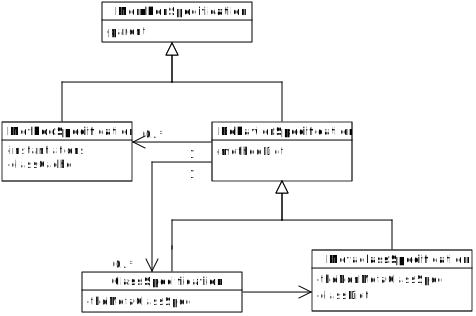
\includegraphics[scale=1]{metamodel.pdf}
	\caption{Meta Model for Nested Classes}
	\label{fig:impl_meta_model}
\end{figure}

\paragraph{Class Specifications}
A class specification describes classes. It has a collection of \texttt{MethodSpecification}s, representing instance methods of the class. Upon instantiation, all method specifications are instantiated within the target class. For every class specification, there is a corresponding method specification containing the source code of the class generator method in the parent's method dictionary. This method specification determines (when executed in the running system) to which class the methods will be added (\emph{target class}). Top-level classes are an exception: they are always a new subclass of the class \texttt{Module}.

\paragraph{Meta Class Specification}
A meta class specification describes meta classes. It has a collection of \texttt{MethodSpecification}s, representing class methods of the class (i.e., instance methods of the meta class). Upon instantiation, all method specifications are instantiated within the targer class' meta class. Consequently, meta classes do not method specifications associated with.

However, meta classes can have nested classes of their own. For every class defined in a meta class, there is a corresponding method specification present in the method dictionary (see previous paragraph).

\paragraph{Method Specification}
A method specification describes methods. It contains the source code of the method and stores information necessary for class caching and UI metadata. Whenever a method specification is instantiated, the method source code is compiled in the target class. 

Note, that different byte code must be generated for different target classes: for example, instance variable reads and write are compiled to parameterized\footnote{There are separate bytecodes for reading the first or second instance variable etc.} \texttt{pushRcvr:} and \texttt{popIntoRcvr:} bytecodes, where instance variables are referenced with their index\footnote{The first instance variable has index 0, second index variable has index 1, etc.}. In addition, the \texttt{outer} and the \texttt{enclosing} keyword must be bound to different method literals, depending on the lexical scope of the class.

\paragraph{Class Initialization}

accessor methods and generator methods, lazy initialization

\section{Anonymous Classes and Subclass Generation}

\section{\texttt{thisOuter} and \texttt{thisScope}}

\section{Class Updates}
using instances weak array on specification

\section{Integration in Squeak}

\subsection{Module Repository}
replacement for Smalltalk dict

\subsection{IDE Support}
works in workspace, test runner. How to write tests? New system browser

\subsection{Debugger}
shows slightly different code (thisContext automatically inserted, generator methods)
% \input{evaluation}
% \chapter{Related Work}
\label{sec:related}

\section{Class Name Clashes}

\subsection{Namespaces/Packages and Class Nesting}
Many programming languages have a concept of namespaces or packages. Classes are typically organized in a package, which is a set of classes. Classes within a package can usually reference each other directly. However, references to classes in other packages typically require imports, aliases, or a fully qualified name. Some programming languages also support class nesting, where the enclosing class creates a namespace for all inner/nested classes.

\paragraph{VisualWorks Namespaces}
VisualWorks is a commerical Smalltalk implementation sold by Cincom and supports namespaces~\cite{brauer2015programming}. A namespace is a container for other namespaces, classes, and shared variables. Since a namespace can be defined within another namespace, VisualWorks allows for a form of hierarchical decomposition. All namespace members (e.g., classes) in the same namespace can be referenced by just writing down their names. All namespace members in other namespaces can be referenced by writing down their fully qualified name, which is the concatenation of all nested namespace names and the name of the class with dots as separators. For example, the fully qualified name of a class \texttt{C1} in namespace \texttt{B} in namespace \texttt{A} is \texttt{A.B.C1}. Relatives name are also supported: for example, \texttt{A.B.C1} can be referenced as \texttt{B.C1} within \texttt{A}.

A namespace can import members from other namespaces by specifying a list of all imports when the namespace is defined~\cite{cincomst}. Wildcard imports are possible, importing all members of a namespace. Imported members can be referenced within a namespace as if they were part of that namespace. A namespace member can also be defined as \emph{private}; such a member cannot be imported, but always has to be referenced using its fully qualified name or using a relative name.

Namespaces are instances of the class \texttt{NameSpace}, which is a subclass of \texttt{Collection}. \texttt{NameSpace} defines a few helper methods to allow for meta programming, such as listing all classes or defining new namespaces or classes within a namespace.

\paragraph{Java Packages and Nested Classes}
The Java programming language has a concept of packages. A package is set of classes, interfaces, and pacckages, and corresponds to a directory on the file system. Classes and interfaces in the same package can be referenced directly using their name. Classes and interfaces in other packages can be referenced using their fully qualified name, which is generated exactly as in VisualWorks. They can also be imported explicitly, making it possible to reference them just using their name; wildcard imports are possible.

Classes and interfaces can be defined as package-public or package-private. Only package-public members can be imported or referenced within members outside of the current package.

Java supports the concept of nested classes: a class can either be a top-level class or a class that is nested within another member. There are four different kinds of nested classes~\cite{Bloch:2008:EJ:1377533}.
\begin{itemize}
	\item \emph{Static member class:} a class that belongs to another class, i.e., it is a static member of another class. It can be accessed like a static variable of the enclosing class. For example, if \texttt{B} is nested in \texttt{A}, it can be referenced with \texttt{A.B}. Messages sent from within the nested class are first looked up in the nested class and its superclass hierarchy, then on the class side of the enclosing class (static methods), and then in the enclosing class' enclosing class (if it is a nested class).
	\item \emph{Nonstatic member class:} a class that belongs to an instance of another class, i.e., it is a nonstatic member of another class. It is similar to a static member class, but the method lookup happens on the instance side of the enclosing class. Every instance of a class has its own nonstatic member classes; however, all of these classes must inherit from a class that can be resolved at compile time. Effectively, all nonstatic member classes are the same, with the only exception that they are bound to different enclosing objects.
	\item \emph{Anonymous class:} a class without a name. In older Java versions, it was frequently used as a substitute for missing block closures. Lambda expressions are available since Java 8, making anonymous classes obsolete in many use cases. Note, that since classes are not first-class objects in Java, it is difficult to pass anonymous classes around and to use them in a different context without using meta programming.
	\item \emph{Local class:} a class that can be defined anywhere where a local variable can be defined. It is the least frequently used kind of classes.
\end{itemize}

Static member classes are similar to packages. By just looking at source code that references a static member class, it is not obvious whether the class is statically nested or contained in a package.

Java imposes certain restrictions on member classes. For example, nonstatic member classes are not allowed to have static member which are not final~\cite{javalang1}. Furthermore, a subclass cannot override a member class definition~\cite{igarashi2002inner}; it can just define its own member class. The difference is that overriding implies late binding, which is not the case in Java. With \emph{Jx}, Nystrom et al. changed the Java language is such a way, that subclasses can enhance member classes~\cite{Nystrom:2004:SEV:1028976.1028986}: the new member class overrides the original one and is always a subclass and a subtype of the member class in the superclass. Jx also allows changing the superclass of a member class in a subclass of the enclosing class, a form of mixin modularity.

\paragraph{Ruby Modules}
Ruby has the concept of classes and modules. Modules are classes which are not instantiable. They can be included in classes and be used as mixins. Modules and classes can be nested in each other, defining a namespace. Classes and modules can be accessed using their fully qualified name, which is the concatenation of their names with two colons as separator. For example, if class \texttt{B} is nested in class \texttt{A}, \texttt{B}'s fully qualified named is \texttt{A::B}. Classes and modules can also be accessed using relative names. For example, when accessing \texttt{A::B}, Ruby first looks for \texttt{A} in the current class/module. If there no such member, it looks in the enclosing class/module.

In Ruby, a class can have methods, variables, and constants. An inner class or module is just a constant defined on the enclosing class. Constants are copied or shared during subclassing. Subclasses can replace inner classes with their own implementation. A nested class/module is always a class-side member of their enclosing class/module (nonstatic member class in Java).

In Ruby, classes and modules can be extended after they have been defined. In case of an accidential class/module name clash, the two (or more) classes/modules are effectively merged. In case of colliding methods, the method that was last seen (read from the file) overwrites all previous definitions. This process is often used deliberately in Ruby, in order change the behavior of a library or application, e.g., to fix a known bug (\emph{monkey patching})~\cite{Benson:2008:AR:1386543}. 

\paragraph{Python Modules}
In Python, every source code file is a module. Modules have to be imported, before they can be used within another module. Members defined in a module can be referenced by concatenating the module name and the name of the member (e.g., class or function) inside the module with a dot as a separator, if the module is imported. It is also possible to import single members from a module with their own name or an alias. These members can be accessed without writing down the module name.

In Python, every directory with a \texttt{\_\_init\_\_.py} source code file is a package. Packages can contain other packages and modules. Packages can be imported just like modules. The fully qualified name of a module is the concatenation of all package names and the module name, with a dot as a separator.

Modules in other packages can be imported by writing their fully qualified name or using a path relative to the current module~\cite{pythonp1}.

Python supports inner classes, but only for readability and understandability reasons, and their usage is not wide-spread. Inner classes are class-side members of the enclosing class. In fact, for every inner class, Python creates an attribute on the enclosing class object with the inner class name as name and the inner class object as value. Since all nested class attributes are copied during subclassing, a subclass shares the same inner classes as the superclass. Redefining an inner class on the superclass simply replaces it. Inner classes do not affect the class lookup: for example, when two inner classes nested on the same level want to reference each other, both have to write their \emph{full path} (i.e., sequence of attribute reads).

Whenever a top-level class is defined and there is already a class with that name in the same module, the new class replaces the existing one.

\subsection{Squeak Environments}
\label{sec:rel_sq_env}

\subsection{Newspeak Modules}


\section{Dependency Management}

\subsection{Metacello}
\label{sec:rel_metacello}

\subsection{Java Class Loader}

\subsection{Separate Compilation}

\subsection{Dependency Injection}
%http://www.jot.fm/issues/issue_2012_04/article3.pdf

\subsection{External Configuration in Newspeak}


\section{Readability and Understandability}

\subsection{Smalltalk Packages}

\subsection{Hierarchical Decomposition}
Java, Python, Ruby, Newspeak, \ldots

\subsection{Information Hiding with Interfaces}


\section{Code Reuse}

\subsection{Multiple Inheritance}

\subsection{Mixins}
Ruby Modules, Python Multiple Inheritance, Newspeak, Jigsaw

\subsection{Traits}
\label{sec:rel_traits}
Squeak implementation

\subsection{Java Generics}
Java generics allow classes and interfaces to be parameterized by one or multiple classes and interfaces for type checking reasons~\cite{bracha2004generics}. Theya are often used together with collections~\cite{Parnin:2011:JGA:1985441.1985446}. Generic parameters are defined as part of the class or interface definition. When a class or interface is used, the programmer can pass classes and interfaces as arguments.

\begin{figure}[!htp]
\begin{lstlisting}
class Array<T> {
    T[] storage;

    public List(int size) {
        storage = /* ??? */;
    }

    T get(int index) {
        return storage[index];
    }

    void set(int index, T value) {
        storage[index] = value;
    }
}

Array<String> arr = new Array<String>(100);
\end{lstlisting}
\caption{Generic array implementation using Java generics}
\label{fig:rel_java_generics}
\end{figure}

Figure~\ref{fig:rel_java_generics} shows how Java generics are used in practise. \texttt{T} is the generic parameter of the class \texttt{Array}. The compiler ensures that only arguments with the correct type \texttt{T} can be passed to \texttt{set()} and knows that \texttt{get()} can only return objects of type \texttt{T}. 

One shortcoming of Java generics is type erasure: generic type information is only known at compile time, but not at runtime. Therefore, Java actually allocates a storage array of type \texttt{Object[]}. Therefore, it is difficult to initialize \texttt{storage} to an array of type \texttt{T}. In fact, the statement \texttt{new T[size]} does not compile. What the programmer could write instead is an unchecked type cast~\cite{nino2007cost}: \texttt{(T[]) new Object[size]}.

\subsection{C++ Templates}

% \input{conclusion}
%

% beispiel.

\chapter{Introduction}

\section{Modularity}

\section{The Squeak Programming Language}
Smalltalk is an object-oriented, class-based programming language and Squeak is a Smalltalk-80 dialect. It was originally developed by Alan Kay, Dan Ingalls, and Adele Goldberg. Dan Ingalls described Smallktalk-80 as a project whose purpose is to ``provide computer support for the creative spirit in everyone.'' In his article ``Design Principles Behind Smalltalk''~\cite{Inga81a}, which appeared in August 1981 in the BYTE Magazine, he mentions some of the most fundamental principles behind the Smalltalk project. Some of these go hand and hand with modularity and can be further supported by a good module system.

\begin{itemize}
	\item ``Personal mastery: If a system is to serve the creative spirit, it must be entirely comprehensible to a single individual.'' A module system can support understandability of a system by breaking up big components into smaller one (\emph{hierarchical decomposition}) and hiding irrelevant implementation details.
	\item ``Factoring: Each independent component in a system would appear in only one place.'' A module system can encourage code reuse by making it easy to store shared behavior and components in a designated place that allows other components to take advantage of it and eliminate code duplication.
	\item ``Modularity: No component in a complex system should depend on the internal details of another component.'' Through information hiding, a module system can encourage programmers not to rely on implementation-specific behavior. A notion of what is considered a public interface can help keeping modules exchangable and increases understandability, since only the public interface should be sufficient to understand what a module is doing.
	\item ``Good Design: A system should be built with a minimum set of unchangable parts; those parts should be as generic as possible.'' Consequently, if we are to create a module system for Smalltalk, that system should build on top of a single fundamental concept, and all features and use cases should evolve out of this concept in a natural way without any special corner cases.
\end{itemize}


\section{Outline of this Work}

\chapter{Modularity Problems in Squeak}
\label{sec:problem}
In this section, we describe and evaluate how Squeak can be used to write modular programs at the moment. Based on our observations and programming experience with Squeak, there are three areas in which we see room for improvement. For every area, we will describe what the problem is and how it is currently solved in Squeak.

\paragraph{Class-based Modularity}
In pure Smalltalk, classes are the highest level of modular units. Classes are first-class objects and can be passed around. This functionality can be used to make behavior interchangable and promotes loose coupling. Classes are Smalltalk's way of sharing behavior with a number of objects, i.e., it is a form of code reuse. Squeak also supports Traits, a design method for composing class of pieces of behavior (see Section~\ref{sec:rel_traits}).

Smalltalk is, as most object-oriented and class-based programming languages, amenable to well-established software design patterns~\cite{Gamma:1995:DPE:186897}, making it easier to write maintainable and understandable code.

\section{Duplicate Class Names}
In Squeak, there can only be only one class with a certain name. Whenever, the programmer tries to add another class with the same name, a conflict occurs. When source code is loaded into the system with the Monticello version control system, the system asks the programmer if the already existing class should be replaced. As a workaround, it is good practice to add unique namespace prefixes to all class names in an application. 

Squeak has packages~\cite{Nierstrasz:2009:SE:1816759}, but these are not used as namespaces. Their purpose is to make it easier to find existing classes (like method protocols). They are also used as deployment units. The programmer does usually not load single classes into the system. Instead, packages (groups of classes) are loaded. 

Squeak environments provide a way to have multiple classes with the same name in one image. However, they suffer from poor tool support and do not integrate well with some of the other goals (e.g., code reuse) for our system. See Section~\ref{sec:rel_sq_env} for a detailed discussion of Squeak environments and why we did not use them in this system.

\paragraph{Example}
\begin{figure}[!htp]
\dirtree{%
.1 \framebox{\textbf{BroBreakout}}.
.2 BroBall.
.2 BroBlock.
.2 BroBoundary.
.2 BroBreakout.
.2 BroExplosion.
.2 BroLevelBuilder.
.2 BroLevelStatistics.
.2 BroLevelStatisticsItem.
.2 BroLevelView.
.2 BroLevelWorld.
.2 BroMenuLabel.
.2 BroMenuView.
.2 \textit{BroPowerup}.
.2 BroPowerupAccelerate.
.2 BroPowerupBall.
.2 BroPowerupDecelerate.
.2 BroPowerupEnlarge.
.2 BroPowerupShrink.
.2 BroRacket.
.2 \textit{BroView}.
.2 BroWelcomeView.
}
\caption[Breakout class structure]{Breakout class structure. All classes have the \texttt{Bro} namespace prefix and are contained in the package \texttt{BroBreakout}.}
\label{fig:conc_breakout}
\end{figure}

Consider the game Breakout (Figure~\ref{fig:conc_breakout}, see also Section~\ref{sec:usecase_hierach_decomp}). This application uses \texttt{Bro} as a prefix for all classes. If we would not use namespace prefixes, generic class names like \texttt{Block} or \texttt{Ball} would be likely to collide with other classes. On the other hand, if all application and library developers adhere to this convention, it is unlikely that class name classes occur.

\section{Dependency Managment}
Dependency management describes the task of keeping track of dependencies and ensuring that required dependencies are available to the application in question. We destinguish between two cases of dependency management: internal dependency management, i.e., the application specifies all dependencies, and external dependency managment (\emph{external configuration}), i.e., user of the application specifies all dependencies. But before managing dependencies, we need a versioning concept that allows us to represent library versions in an image.

\paragraph{Versioning}
There are situations when it is useful to have multiple versions of the same library in one image; for example, if there are two different applications installed and both require the same library, but in different versions. Old versions of a library might have bugs that an application has to work around. The application might then not work with a newer library, where the bug is fixed. Furthermore, the public API of a library might change with new versions, especially if it is a new major version.

Therefore, we need a versioning mechanism in \msname, that helps us to store and reference different versions of the same application or library in one image. Part of this mechanism must be a way to develop new library versions, and a mechanism to reference a certain version.

\paragraph{Internal Dependency Management}
In this case, every application or library specifies itself which dependencies (and their versions) it depends on. The application effectively maintains the list of dependencies itself. Consequently, the application is coupled to its dependencies and cannot be used with different versions or implementations without changing its source code.

\paragraph{External Configuration}
In this case, the dependency management is delegated to the client of an application or library. What the application specifies is that it requires some dependency implementing a certain interface, but not what exact dependency it is exactly or in what version. This mechanism is also called \emph{dependency injection} and used heavily in the Java world~\cite{Prasanna:2009:DI:1795686}. Dependency injection is also known as \emph{inversion of control}~\cite{fowlerioc}, because it inverts the control of dependencies: it is shifted from the application or library in question to the user/client. External configuration is beneficial for modularity, because it supports loose coupling of application and dependencies. This, in turn, promotes understandability, maintainablity, and exchangability (code reuse), because an application cannot rely on implementation details of a loosely bound dependency.

\paragraph{Dependency Management in Squeak}
In Squeak, there can currently only be one version of a library or application installed at a time. Monticello is used a source code management system and can be used to load new versions of the source code into an image. Metacello is a package management system (see Section~\ref{sec:rel_metacello}), similar to Maven in Java. Every Metacello package has a configuration class containing a list of external dependencies and internal packages to load for every version, along with the location of an external repository where the packages should be loaded from~\cite{metacellodraft}.

External configuration can simulated in Smalltalk by writing class constructors that accept other dependencies as parameters. These dependencies should then be stored in instance variables and only be accessed using instance variables. However, this technique has two pitfalls. Firstly, dependencies have to be forwarded to all other classes, resulting in boilerplate code. Secondly, only instance methods can benefit from external configuration, because class methods are shared among instances (configurations) of the class.

\section{Hierarchical Decomposition}
Smalltalk packages allow the programmer to group together what belongs together~\cite{Eckel:2002:TJ:579108}. This is especially useful in big projects with many classes and allows for a form of modular decomposition. Different criterias for modular decomposition have been proposed: e.g., functional decompositon (making every step in the \emph{flowchart} a module) or information hiding~\cite{Parnas:1972:CUD:361598.361623}. The following list shows some benefits of good modular decomposition.

\begin{itemize}
	\item Changability (continuity): only few classes are affected when changing a detail.
	\item Independent development: classes can be developed in parallel.
	\item Understandability: in order to understand the behavior of a class, it is sufficient to read code within that class.
\end{itemize}

What we want to achieve is hierarchical decomposition~\cite{Blume:1999:HM:325478.325518}, which is in a basic form realized in Java packages, Ruby namespace module, or Python modules. It can increase comprehensibility of the overall system when it acts as some kind of decision tree that helps the programmer finding a submodule corresponding to a certain functionality in an unknown application. 

It also allows for fine-grained dependency management: for example, it is considered good practice in many programming languages to keep import statements as small as possible. Import statements also act as documentation, giving the reader of the source code a rough idea of what the source code might do. Furthermore, if a functionality is nested in a submodule, it is likely that it is written in a more general way, such that it might be reused elsewhere in the application without bigger changes.

If the source code is functionally decomposed in a hierarchical way~\cite{Tsui:2009:ESE:1823101}, it is also easier to understand single submodules of the system. The reader of the source code might only be interested in a certain level of detail (e.g., no low-level functionality), and then skip deeply nested submodules~\cite{hierarch1} (information hiding or abstraction). Since in functional decomposition, the purpose of nested modules is usually only to serve their enclosing modules, readers can start off with a high-level idea of the module is doing by going through the first few levels of nesting, and dive in deeper as needed.

Therefore, one of the requirements for our system is to provide a mechanism for hierarchical code decomposition that is more than just one level deep (Smalltalk packages).

\paragraph{Example}
Consider the game SpaceCleanup, which is a simple bomberman clone (Figure~\ref{fig:prob_space_cleanup_org}, see also Section~\ref{sec:usecase_hierach_decomp}). The source code for this game is organized in multiple packages. For example, all items in the game are grouped in the package \texttt{SpaceCleanup-Items}. Besides this obvious single-level decomposition, the game is actually already functionally decomposed in a hierarchical way. For example, \texttt{ScuLevel} represents a level in the game. A level consists of multiple tiles (\texttt{ScuTile}). A tile cannot exist without a level; its sole purpose is to serve \texttt{ScuLevel}. Similarly, items always belong to a tile and cannot be used without a tile. All in all, SpaceCleanup is already functionally decomposed, but this decomposition is not fully reflected in the class organization.

\begin{figure}[!htp]
\dirtree{%
.1 \framebox{\textbf{SpaceCleanup-Core}}.
.2 ScuEventDispatcher.
.2 ScuGame.
.2 ScuGameBuildState.
.2 ScuGameConfigState.
.2 ScuGameOverState.
.2 ScuGamePausedState.
.2 ScuGameRunningState.
.2 \textit{ScuGameState}.
.2 ScuGameWonState.
.2 \textit{ScuMonsterStrategy}.
.2 ScuMonsterRandomStrategy.
.2 ScuMonsterToPlayerStrategy.
}
\vspace{10pt}
\dirtree{%
.1 \framebox{\textbf{SpaceCleanup-Items}}.
.2 ScuBucket.
.2 \textit{ScuDestructibleItem}.
.2 ScuFloor.
.2 \textit{ScuItem}.
.2 ScuMonster.
.2 \textit{ScuMovingItem}.
.2 ScuPickUpItem.
.2 ScuPlayer.
.2 ScuPortal.
.2 ScuSlime.
.2 ScuWall.
.2 ScuWater.
}
\vspace{10pt}
\dirtree{%
.1 \framebox{\textbf{SpaceCleanup-Level}}.
.2 ScuLevel.
.2 \textit{ScuLevelBuilder}.
.2 ScuGridPatternLevelBuilder.
.2 ScuRandomLevelBuilder.
.2 ScuTile.
}
\vspace{10pt}
\dirtree{%
.1 \framebox{\textbf{SpaceCleanup-Resources}}.
.2 ScuResourceManager.
}
\vspace{10pt}
\dirtree{%
.1 \framebox{\textbf{SpaceCleanup-UI}}.
.2 ScuCheatWindow.
.2 ScuConfigurationWindow.
.2 ScuControls.
.2 ScuGameInformation.
}
\caption[SpaceCleanup class organization]{SpaceCleanup class organization. All classes have the \texttt{Scu} namespace prefix and are grouped in five packages, according to their responsibilities.}
\label{fig:prob_space_cleanup_org}
\end{figure}


%\section{Code Reuse}
%share behavior among multiple classes

\chapter{Related Work}
\label{sec:related}

\section{Class Name Clashes}

\subsection{Namespaces/Packages and Class Nesting}
Many programming languages have a concept of namespaces or packages. Classes are typically organized in a package, which is a set of classes. Classes within a package can usually reference each other directly. However, references to classes in other packages typically require imports, aliases, or a fully qualified name. Some programming languages also support class nesting, where the enclosing class creates a namespace for all inner/nested classes.

\paragraph{VisualWorks Namespaces}
VisualWorks is a commerical Smalltalk implementation sold by Cincom and supports namespaces~\cite{brauer2015programming}. A namespace is a container for other namespaces, classes, and shared variables. Since a namespace can be defined within another namespace, VisualWorks allows for a form of hierarchical decomposition. All namespace members (e.g., classes) in the same namespace can be referenced by just writing down their names. All namespace members in other namespaces can be referenced by writing down their fully qualified name, which is the concatenation of all nested namespace names and the name of the class with dots as separators. For example, the fully qualified name of a class \texttt{C1} in namespace \texttt{B} in namespace \texttt{A} is \texttt{A.B.C1}. Relatives name are also supported: for example, \texttt{A.B.C1} can be referenced as \texttt{B.C1} within \texttt{A}.

A namespace can import members from other namespaces by specifying a list of all imports when the namespace is defined~\cite{cincomst}. Wildcard imports are possible, importing all members of a namespace. Imported members can be referenced within a namespace as if they were part of that namespace. A namespace member can also be defined as \emph{private}; such a member cannot be imported, but always has to be referenced using its fully qualified name or using a relative name.

Namespaces are instances of the class \texttt{NameSpace}, which is a subclass of \texttt{Collection}. \texttt{NameSpace} defines a few helper methods to allow for meta programming, such as listing all classes or defining new namespaces or classes within a namespace.

\paragraph{Java Packages and Nested Classes}
The Java programming language has a concept of packages. A package is set of classes, interfaces, and pacckages, and corresponds to a directory on the file system. Classes and interfaces in the same package can be referenced directly using their name. Classes and interfaces in other packages can be referenced using their fully qualified name, which is generated exactly as in VisualWorks. They can also be imported explicitly, making it possible to reference them just using their name; wildcard imports are possible.

Classes and interfaces can be defined as package-public or package-private. Only package-public members can be imported or referenced within members outside of the current package.

Java supports the concept of nested classes: a class can either be a top-level class or a class that is nested within another member. There are four different kinds of nested classes~\cite{Bloch:2008:EJ:1377533}.
\begin{itemize}
	\item \emph{Static member class:} a class that belongs to another class, i.e., it is a static member of another class. It can be accessed like a static variable of the enclosing class. For example, if \texttt{B} is nested in \texttt{A}, it can be referenced with \texttt{A.B}. Messages sent from within the nested class are first looked up in the nested class and its superclass hierarchy, then on the class side of the enclosing class (static methods), and then in the enclosing class' enclosing class (if it is a nested class).
	\item \emph{Nonstatic member class:} a class that belongs to an instance of another class, i.e., it is a nonstatic member of another class. It is similar to a static member class, but the method lookup happens on the instance side of the enclosing class. Every instance of a class has its own nonstatic member classes; however, all of these classes must inherit from a class that can be resolved at compile time. Effectively, all nonstatic member classes are the same, with the only exception that they are bound to different enclosing objects.
	\item \emph{Anonymous class:} a class without a name. In older Java versions, it was frequently used as a substitute for missing block closures. Lambda expressions are available since Java 8, making anonymous classes obsolete in many use cases. Note, that since classes are not first-class objects in Java, it is difficult to pass anonymous classes around and to use them in a different context without using meta programming.
	\item \emph{Local class:} a class that can be defined anywhere where a local variable can be defined. It is the least frequently used kind of classes.
\end{itemize}

Static member classes are similar to packages. By just looking at source code that references a static member class, it is not obvious whether the class is statically nested or contained in a package.

Java imposes certain restrictions on member classes. For example, nonstatic member classes are not allowed to have static member which are not final~\cite{javalang1}. Furthermore, a subclass cannot override a member class definition~\cite{igarashi2002inner}; it can just define its own member class. The difference is that overriding implies late binding, which is not the case in Java. With \emph{Jx}, Nystrom et al. changed the Java language is such a way, that subclasses can enhance member classes~\cite{Nystrom:2004:SEV:1028976.1028986}: the new member class overrides the original one and is always a subclass and a subtype of the member class in the superclass. Jx also allows changing the superclass of a member class in a subclass of the enclosing class, a form of mixin modularity.

\paragraph{Ruby Modules}
Ruby has the concept of classes and modules. Modules are classes which are not instantiable. They can be included in classes and be used as mixins. Modules and classes can be nested in each other, defining a namespace. Classes and modules can be accessed using their fully qualified name, which is the concatenation of their names with two colons as separator. For example, if class \texttt{B} is nested in class \texttt{A}, \texttt{B}'s fully qualified named is \texttt{A::B}. Classes and modules can also be accessed using relative names. For example, when accessing \texttt{A::B}, Ruby first looks for \texttt{A} in the current class/module. If there no such member, it looks in the enclosing class/module.

In Ruby, a class can have methods, variables, and constants. An inner class or module is just a constant defined on the enclosing class. Constants are copied or shared during subclassing. Subclasses can replace inner classes with their own implementation. A nested class/module is always a class-side member of their enclosing class/module (nonstatic member class in Java).

In Ruby, classes and modules can be extended after they have been defined. In case of an accidential class/module name clash, the two (or more) classes/modules are effectively merged. In case of colliding methods, the method that was last seen (read from the file) overwrites all previous definitions. This process is often used deliberately in Ruby, in order change the behavior of a library or application, e.g., to fix a known bug (\emph{monkey patching})~\cite{Benson:2008:AR:1386543}. 

\paragraph{Python Modules}
In Python, every source code file is a module. Modules have to be imported, before they can be used within another module. Members defined in a module can be referenced by concatenating the module name and the name of the member (e.g., class or function) inside the module with a dot as a separator, if the module is imported. It is also possible to import single members from a module with their own name or an alias. These members can be accessed without writing down the module name.

In Python, every directory with a \texttt{\_\_init\_\_.py} source code file is a package. Packages can contain other packages and modules. Packages can be imported just like modules. The fully qualified name of a module is the concatenation of all package names and the module name, with a dot as a separator.

Modules in other packages can be imported by writing their fully qualified name or using a path relative to the current module~\cite{pythonp1}.

Python supports inner classes, but only for readability and understandability reasons, and their usage is not wide-spread. Inner classes are class-side members of the enclosing class. In fact, for every inner class, Python creates an attribute on the enclosing class object with the inner class name as name and the inner class object as value. Since all nested class attributes are copied during subclassing, a subclass shares the same inner classes as the superclass. Redefining an inner class on the superclass simply replaces it. Inner classes do not affect the class lookup: for example, when two inner classes nested on the same level want to reference each other, both have to write their \emph{full path} (i.e., sequence of attribute reads).

Whenever a top-level class is defined and there is already a class with that name in the same module, the new class replaces the existing one.

\subsection{Squeak Environments}
\label{sec:rel_sq_env}

\subsection{Newspeak Modules}


\section{Dependency Management}

\subsection{Metacello}
\label{sec:rel_metacello}

\subsection{Java Class Loader}

\subsection{Separate Compilation}

\subsection{Dependency Injection}
%http://www.jot.fm/issues/issue_2012_04/article3.pdf

\subsection{External Configuration in Newspeak}


\section{Readability and Understandability}

\subsection{Smalltalk Packages}

\subsection{Hierarchical Decomposition}
Java, Python, Ruby, Newspeak, \ldots

\subsection{Information Hiding with Interfaces}


\section{Code Reuse}

\subsection{Multiple Inheritance}

\subsection{Mixins}
Ruby Modules, Python Multiple Inheritance, Newspeak, Jigsaw

\subsection{Traits}
\label{sec:rel_traits}
Squeak implementation

\subsection{Java Generics}
Java generics allow classes and interfaces to be parameterized by one or multiple classes and interfaces for type checking reasons~\cite{bracha2004generics}. Theya are often used together with collections~\cite{Parnin:2011:JGA:1985441.1985446}. Generic parameters are defined as part of the class or interface definition. When a class or interface is used, the programmer can pass classes and interfaces as arguments.

\begin{figure}[!htp]
\begin{lstlisting}
class Array<T> {
    T[] storage;

    public List(int size) {
        storage = /* ??? */;
    }

    T get(int index) {
        return storage[index];
    }

    void set(int index, T value) {
        storage[index] = value;
    }
}

Array<String> arr = new Array<String>(100);
\end{lstlisting}
\caption{Generic array implementation using Java generics}
\label{fig:rel_java_generics}
\end{figure}

Figure~\ref{fig:rel_java_generics} shows how Java generics are used in practise. \texttt{T} is the generic parameter of the class \texttt{Array}. The compiler ensures that only arguments with the correct type \texttt{T} can be passed to \texttt{set()} and knows that \texttt{get()} can only return objects of type \texttt{T}. 

One shortcoming of Java generics is type erasure: generic type information is only known at compile time, but not at runtime. Therefore, Java actually allocates a storage array of type \texttt{Object[]}. Therefore, it is difficult to initialize \texttt{storage} to an array of type \texttt{T}. In fact, the statement \texttt{new T[size]} does not compile. What the programmer could write instead is an unchecked type cast~\cite{nino2007cost}: \texttt{(T[]) new Object[size]}.

\subsection{C++ Templates}

\chapter{Nested Class Modularity in Squeak}
\label{sec:concept}
In this chapter, we describe the main concept of this work: classes as class members. Similar concepts are part of programming languages like Java, Ruby, Python, and Newspeak. Our concept follows closely the Newspeak notion of nested classes, but without making invasive changes to the Smalltalk programming language.

\section{Nested Classes}
In Smalltalk, every object is an instance of a class, defining the object's instance variables and the messages it understands. Consequently, a class is also an instance of its so-called meta class. Every meta class is an instance of \texttt{Metaclass} (Figure~\ref{fig:impl_squeak_meta}). In the remainder of this work, we denote the meta class of a class \texttt{C} by \texttt{C class}. Every Smalltalk image has a \texttt{globals} dictionary\footnote{Squeak also supports \emph{environments}, effectively making it possible to compile methods in the context of another \texttt{globals} dictionary. See Section~\ref{sec:rel_sq_env} for more details.}, mapping symbols to class objects, so that references to classes can be resolved at compile time. This implies that all references to classes are early bound.

\begin{wrapfigure}{l}{0.5\textwidth}
	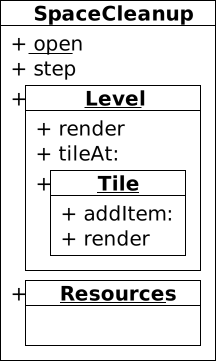
\includegraphics[scale=0.75]{nested_notation.pdf}
	\centering
	\caption[Example: Nested classes]{Example: nested classes. A class can have class-side member classes.}
	\label{fig:concept_nested_notation}
\end{wrapfigure}

\msname extends the Smalltalk class organization as follows: in addition to regular methods, we introduce the concept of \emph{class generator methods}. Such a method generates a class and is associated with a set $I$ of instance methods and a set $C$ of class methods. Whenever the method is invoked, the system first executes the method body, then adds $I$ to the resulting class and $C$ to the resulting meta class, and finally returns the resulting class. For performance reasons, \msname also caches the result, meaning that a class is not generated twice.

\paragraph{Details}
Class generator methods are only allowed as class-side methods. Instance-side class generator methods seem to provide neglectable benefits and make the implementation of our system more complicated. We discuss instance-side class generator methods in more detail in the Section~\ref{sec:future_inst_side}.

A class generated by a class generator method is anonymous: it is not listed in the \texttt{globals} dictionary and can only be referenced using message sends to its enclosing class\footnote{It can also be referenced by sending the \texttt{class} message to one of its instances}. Consequently, its name is a concatenation of all class names on the path from the top-level class to the class in question.


\paragraph{Notation and Example}
Figure~\ref{fig:concept_nested_notation} shows an example of nested classes in \msname. \texttt{A} is a top-level class, i.e., it is part of the \texttt{globals} dictionary and known everywhere in the system; it can be referenced by just writing the identifier \texttt{A}. \texttt{A} has one instance method \texttt{m2} and two class methods \texttt{m1} and \texttt{B}. In accordance with UML notation, class-side method selectors are underlined. 

\texttt{A class>>B} is a class generator method that is associated with a set of instance methods $\{\}$ and a set of class methods $\{\mbox{\texttt{foo}, \texttt{C}}\}$. The name of the class it generates is \texttt{A B}, which is in that case also a valid Smalltalk code expression that evaluates to the generated class. \texttt{A class>>B class>>C} is a class generator method that generates \texttt{A B C}. Note, that we use the \texttt{>>} notation to not only reference methods but also the classes they generate, in case they are class generator methods.

Top-level classes are called \emph{modules}. All other classes are called \emph{nested classes}. The class in which an other class is nested is called the \emph{enclosing class}.

%\begin{figure}[!htp]
%	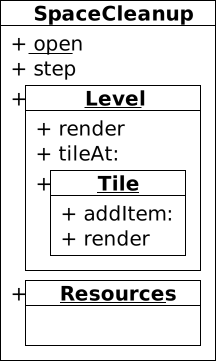
\includegraphics[scale=0.5]{nested_notation.pdf}
%	\centering
%	\caption{Nested Classes Example}
%	\label{fig:concept_nested_notation}
%\end{figure}

\section{Accessing the Lexical Scope}
\begin{wrapfigure}{l}{0.5\textwidth}
	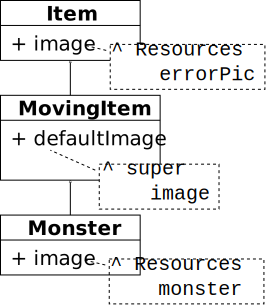
\includegraphics[scale=0.75]{super_binding.pdf}
	\centering
	\caption[Example: Binding of \texttt{super}]{Example: Binding of \texttt{super}. The method lookup starts at the superclass of the calling method's class.}
	\label{fig:concept_super_binding}
\end{wrapfigure}
It is sometimes necessary to access a method's lexical scope (i.e., the enclosing classes), in order to send messages to enclosing classes. For this reason, our system introduces new keywords, in addition to \texttt{self} and \texttt{super}, which are already present in every Smalltalk dialect. Figure~\ref{fig:concept_keywords} gives an overview of all method lookup-related keywords in the system.

\begin{figure}[!htp]
	\centering
	
\includegraphics[scale=1]{lookup_keywords.pdf}
	\caption[Keywords for superclass and lexical scope access]{Keywords for superclass and lexical scope access. The lookup starts at \texttt{self}, and continues with the lexical scope.}
	\label{fig:concept_keywords}
\end{figure}

\subsection{\texttt{self} Keyword}
This keyword is used make a message send within an object. The receiver is the same object as the sender and the lookup starts at the (polymorphic) class of the receiver. If that class does not provide a corresponding method, the lookup continues in the superclass hierarchy. If no class in the superclass hierarchy has a corresponding method, a \texttt{MethodNotUnderstood} error is raised.

\subsection{\texttt{super} Keyword}
This keyword is also used to make a message send within an object. Again, the receiver is the same object as the sender, but the lookup starts at the superclass of the sender's method class. Note, that \texttt{super} is bound to the superclass of the method class, not the superclass of the receiver's class. For example, in Figure~\ref{fig:concept_super_binding}, \texttt{C new bar} returns \texttt{1}, because, in \texttt{B>>bar}, \texttt{super} is bound to \texttt{A}, even though the receiver \texttt{C new} is an instance of \texttt{C}.

\subsection{\texttt{enclosing} Keyword}
This keyword is used to make a message send to the class that contains the current class. Consider, for example, that we want to send a message \texttt{foo} to class \texttt{A B} within \texttt{A class>>B class>>C class>>m4} in Figure~\ref{fig:concept_nested_notation}. Either one of the following two statements works in this case\footnote{The enclosing class of an object that is not a class is its class' enclosing class.}.

\begin{itemize}
	\item \texttt{A B foo.}
	\item \texttt{enclosing foo.}
\end{itemize}

\texttt{enclosing} is a keyword that evaluates to the method owner's enclosing class upon method compilation. Note, that \texttt{enclosing} is bound to the method's lexical scope, not the receiver class' lexical scope.

Figure~\ref{fig:concept_lexical_thisouter} illustrates how \texttt{enclosing} is bound. In \texttt{B1 class>>C class>>bar1}, \texttt{enclosing} is bound to \texttt{B1}. In contrast, \texttt{B2 class>>C class>>bar2} binds \texttt{enclosing} to \texttt{B2}. Consequently, \texttt{B1 C bar1} calls \texttt{B1 foo} and so does \texttt{B2 C bar1}, even though the receiver of \texttt{bar1} is an instance of \texttt{B2 C class} and not \texttt{B1 C class} in the latter case. Note, that \texttt{B2 C bar2} calls \texttt{B2 foo}, because \texttt{bar2}'s lexically enclosing class is \texttt{B2}.

\begin{figure}[!htp]
	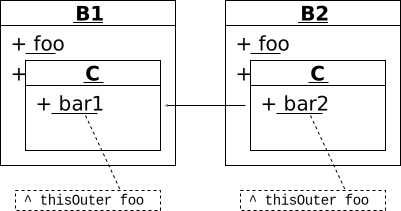
\includegraphics[scale=0.75]{nested_lexical1.pdf}
	\centering
	\caption[Example: Binding of \texttt{enclosing}]{Example: Binding of \texttt{enclosing}. The keyword is bound to enclosing class of the class where the method containing the keyword is contained.}
	\label{fig:concept_lexical_thisouter}
\end{figure}

Note, that \texttt{enclosing} can be used for meta programming purposes; however, it should be avoided in general, because it can lead to fragile code that makes too many assumptions about the structure of the class nesting. A later refactoring could then lead to broken code. Probably for the same reason, Smalltalk does not have a \texttt{super} keyword that does the lookup only in the superclass\footnote{However, there is a method \texttt{Class>>superclass}.} (single-level super). \msname provides a \texttt{scope} keyword that should be used instead.

\subsection{\texttt{enclosing} Method}
In addition to \texttt{enclosing}, every class in the system has a method \texttt{enclosing} that returns the enclosing class (\emph{owner}) of the receiver, making it possible to send messages to enclosing classes which are more than one level away. If, for example, in Figure~\ref{fig:concept_nested_notation}, \texttt{A class>>B class>>C>>bar} wants to send the message \texttt{m1} to \texttt{A}, either one of the following two statements works.

\begin{itemize}
	\item \texttt{A m1.}
	\item \texttt{enclosing enclosing m1.}
\end{itemize}

Again, the method \texttt{enclosing} should be avoided in general, but is useful to implement parts of our system with code written in the system itself and for meta programming. The statement \texttt{enclosing enclosing} would be somewhat similar to a \texttt{super super} statement. Arguably, this can result in verbose and complicated code, and is at the very least questionable with regards to the law of demeter. Note, that, in contrast to the \texttt{outer} keyword, the message send of \texttt{enclosing} in \texttt{enclosing} is no longer bound to the lexical scope of the method.

\subsection{\texttt{outer} Keyword}
\label{sec:concept_outer}
This keyword is used to make a message send to classes in the lexical scope. Whenever a message is sent to \texttt{outer}, the message is first interpreted as a send to \texttt{enclosing}. If that message send fails, the message is sent to the second-level enclosing class in the current lexical scope. Eventually, the message is sent to a top-level class, if no other class understands the message. If even that message send is not understood, the selector is looked up in the \texttt{globals} dictionary. If the selector is absent, a \texttt{MessageNotUnderstood} error is raised.

\texttt{outer} is similar to \texttt{super}, with the difference that \texttt{outer} does a horizontal lookup (lexical scope) and \texttt{super} does a vertical lookup (superclass chain). Note, that messages sent to \texttt{outer} are sent to an object different from \texttt{self}.

\paragraph{Example}
Figure~\ref{fig:concept_outer_1} illustrates how message sends to \texttt{outer} are looked up. Consider, for example, that the method \texttt{foo} in \texttt{A1 B C} calls \texttt{outer bar}. Both \texttt{A1 B C foo} and \texttt{A2 B C foo} call \texttt{A1 class>>bar} in this case, because \texttt{outer} is bound to the lexical scope of the method.

Figure~\ref{fig:concept_outer_2} shows why it is important that \texttt{outer} is bound to the lexical scope. In this example, \texttt{D B2} is a subclass of \texttt{A B1}. If the \texttt{outer} lookup simply traversed the chain of enclosing classes, i.e., first lookup in \texttt{enclosing}, then \texttt{enclosing enclosing}, etc., the message send of \texttt{bar} would fail in \texttt{D B2 C foo}. As another consequence, a nested class might then no longer be able to access a class defined in an enclosing class if the nested class is subclassed and nested in a different enclosing class, since classes are accessed using message sends.

\begin{figure}[!htp]
\begin{subfigure}[b]{\textwidth}
	\centering
	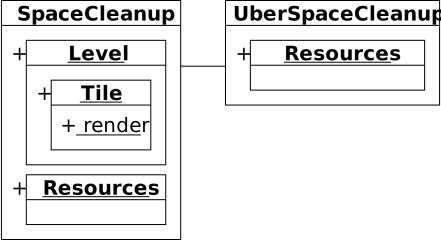
\includegraphics[scale=0.75]{outer_keyword.pdf}
	\caption{Subclassed top-level class}
	\label{fig:concept_outer_1}
\end{subfigure}

\vspace{15pt}

\begin{subfigure}[b]{\textwidth}
	\centering
	\includegraphics[scale=0.75]{outer_keyword_2.pdf}
	\caption{Subclassed nested class with different enclosing class}
	\label{fig:concept_outer_2}
\end{subfigure}

\caption[Example: \texttt{outer} keyword]{Example: \texttt{outer} keyword. Message sends to \texttt{outer} are looked up with respect to the lexical scope of the method, instead of following the chain of enclosing classes (owner hierarchy).}
\end{figure}

%The method \texttt{enclosing} can be used to traverse the the lexical scope of a class. Arbitrarily many \texttt{enclosing} sends can be chained, as long as the respective receiver still has an enclosing class and is, therefore, not a top-level class. Arguably, this can result in verbose and complicated code, and is at the very least questionable with regards to the law of demeter.

%In addition to \texttt{enclosing}, \msname provides the \texttt{outer} keyword, bound to the method's lexical scope. 

% If that message send fails, the message is sent to \texttt{enclosing enclosing}, and, eventually, to the top-level class, if no other class in the lexical scope understands the message. 

\subsection{\texttt{scope} Keyword}
This keyword combines \texttt{super} and \texttt{outer}: a message sent to \texttt{scope} is first treated as a \texttt{self} send. If the message is not understood, it is treated as an \texttt{outer} send.

\msname essentially first looks up the methods in \texttt{self}, then in the superclass hierarchy, and then in the lexical scope. This is how the method lookup in Java works, also known as \emph{comb semantics}~\cite{bracha2007interaction}. Newspeak uses a different lookup: it first looks for a method in the receiver's class, then in the lexical scope, and finally in superclass hierarchy~\cite{bracha:modules_as_objects}.

%The statement \texttt{enclosing enclosing m1} in the previous example can also be written as \texttt{scope m1}. If the method \texttt{m1} would now be moved to its enclosing class (if it had one), the lookup would still succeed. However, \texttt{scope} exposes the risk of accidentially capturing method names in superclasses or the lexical chain.

\subsection{Implicit \texttt{scope} Receiver}
In \msname, references to globals are in fact message sends with \texttt{scope} as implicit receiver. This makes it easier for Smalltalk programmers to write code in \msname, even if they do not know about \texttt{enclosing} and \texttt{scope}. It also makes the code less verbose and easier to read.

Whenever code references an identifier that is not a temporary variable, not an instance variable, and not a \emph{special} object/keyword\footnote{\texttt{self}, \texttt{super}, \texttt{thisContext}, \texttt{scope}, \texttt{outer}, \texttt{enclosing}}, the compiler replaces that identifier with a message send to \texttt{scope}.

Consider, for example, that we want to reference class \texttt{A B} within \texttt{A class>>B class>>C>>bar} in Figure~\ref{fig:concept_nested_notation}. Either one of the following two statements works in this case.

\begin{itemize}
	\item \texttt{A B.}
	\item \texttt{enclosing.}
	\item \texttt{enclosing enclosing B.}
	\item \texttt{outer B.}
	\item \texttt{scope B.}
	\item \texttt{B.}
\end{itemize}

In this example, we used the implicit \texttt{scope} receiver for class lookup, which is in our opinion the most useful case. However, any unary method in \texttt{self}, the lexical scope, or the superclass hierarchy can in fact be looked up this way. One can argue that this is bad practice and should be forbidden for methods that are not class generator methods. However, it is allowed in Newspeak and other programming languages like Java, and seems to work well. Note, that only unary messages can have an implicit \texttt{scope} receiver, since we would have to change the Smalltalk syntax, otherwise.

\section{Parameterized Classes}
All examples shown in the previous sections use unparameterized classes, i.e., class generator methods are always unary. Class generator methods can, however, also have binary selectors or selectors with a higher arity. For memory conservation reasons, these classes are then no longer cached.

\begin{wrapfigure}{l}{0.5\textwidth}
	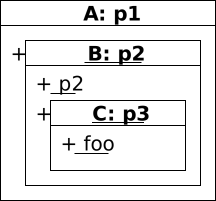
\includegraphics[scale=0.75]{nested_notation_params.pdf}
	\centering
	\caption[Example: Parameterized classes]{Example: Parameterized classes. A class can have parameters accessible with message sends	 to \texttt{enclosing}.}
	\label{fig:concept_param_classes}
\end{wrapfigure}

Parameterized classes can be used to make modules externally configurable or to implement mixins. We will present some conrete use cases in Section~\ref{sec:usecases}.

The arguments passed to a parameterized class generator method are considered when a message is sent to \texttt{enclosing}. At first, the system tries to send the message to the enclosing class. If that fails, \msname checks if the selector corresponds to one of the parameter names in the enclosing class' class generator method.

Consider, for example, that method \texttt{A: class>>B: class>>C: class>>foo} in Figure~\ref{fig:concept_param_classes} contains the following statements.
\begin{itemize}
	\item \texttt{scope p3}: method lookup succeeds in \texttt{A: class>>B: class>>C:} and returns the class parameter \texttt{p3}.
	\item \texttt{scope p2}: method lookup succeeds in \texttt{A: class>>B:} and calls the method \texttt{p2}, which shadows the class parameter \texttt{p2}.
	\item \texttt{scope p1}: method lookup succeeds in \texttt{A:} and returns the class parameter \texttt{p1}.
\end{itemize}

\section{Inheriting Nested Classes}
\label{sec:concept_inh_nested_cl}
Nested classes are accessed using methods returning the generated class. They are similar to class instance variables in a sense that nested classes belong to the enclosing class object. Therefore, a subclass of the enclosing class has its own nested class, i.e., the nested classes might have the same methods and variables declared, but they are different objects. Nested classes can be overridden in subclasses of enclosing classes, just as regular methods can be overridden. The following paragraphs give an overview of how a subclass of an enclosing class can customize the nested class.

\paragraph{Override with Nested Class}
A subclass of an enclosing class can define a new nested class. The programmer simply adds a new class generator method with the same selector to the subclass. The superclass will keep using the old nested class, whereas the subclass will use the new one, because the method lookup ends in the subclass when the corresponding class accessor method is found. The new nested class will only have the methods defined for the subclass' nested class and not inherit or copy any methods from the superclass' nested class.

\paragraph{Override with Regular Method}
A subclass of an enclosing class can replace (override) a nested class with a regular method. The programmer simply adds a new method which is not a class generator method to the subclass.

\paragraph{Extend Inherited Nested Class without Subclassing}
A subclass can extend the inherited nested class, i.e., the nested class in the subclass will have the same superclass as the nested class in the superclass. However, the nested class in the subclass will have all methods defined for the nested class in the superclass and additionally all methods defined for the nested class in the subclass. Duplicate methods will be replaced, similarly to extension methods in Squeak.

\begin{figure}[!htp]
\begin{subfigure}[b]{\textwidth}
	\centering
	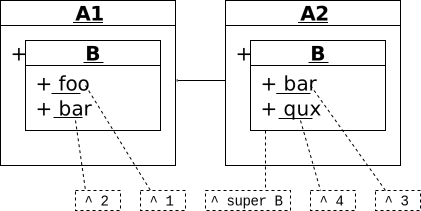
\includegraphics[scale=0.75]{nested_super_1.pdf}
	\caption{Extending inherited nested classing}
	\label{fig:impl:extend_inherited_class}
\end{subfigure}

\vspace{15pt}

\begin{subfigure}[b]{\textwidth}
	\centering
	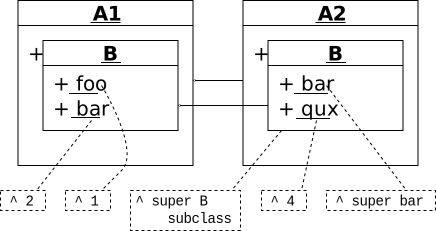
\includegraphics[scale=0.75]{nested_super_2.pdf}
	\caption{Subclassing inherited nested classing}
	\label{fig:impl:subclass_inherited_class}
\end{subfigure}

\caption[Example: Extending/subclassing nested classes]{Example: Extending and subclassing nested classes. Subclassing inherited nested classes leads to parallel class hierarchies.}
\end{figure}

Figure~\ref{fig:impl:extend_inherited_class} shows an example of a nested class extension. Class \texttt{A2} is a subclass of \texttt{A1}, which defines a nested class \texttt{B}. Therefore, both classes \texttt{A1} and \texttt{A2} have a nested class \texttt{B}. \texttt{A2} extends \texttt{B} by perfoming a super call. The following list gives an overview of how the classes \texttt{B} behave.

\begin{itemize}
	\item \texttt{A1 B foo}: returns 1.
	\item \texttt{A1 B bar}: returns 2.
	\item \texttt{A1 B qux}: raises \texttt{MessageNotUnderstood}, because \texttt{qux} is not defined on \texttt{A1 B}.
	\item \texttt{A2 B foo}: returns 1, because \texttt{A2 B} has all methods defined for \texttt{A1 B}.
	\item \texttt{A2 B bar}: returns 3, because that method was replaced in \texttt{A2 B}.
	\item \texttt{A2 B qux}: returns 4.
\end{itemize}

Note, that \texttt{A1 B} and \texttt{A2 B} have the same superclass, but are different class objects. \texttt{A2 B} is \emph{not} a subclass of \texttt{A1 B}. When \texttt{A2 B} is invoked for the first time, \msname first generates the class \texttt{A1 B} (because of the \texttt{super} call) and caches it for \texttt{A2 B}\footnote{Caches are receiver-specific.}. That class is then \emph{reinitialized} according to \texttt{A2 B} (without making a subclass), i.e., all methods defined for \texttt{A2 B} are added. A subsequent call to \texttt{A1 B} will not return the previous generated and extended class for \texttt{A2}, because the class cache works on a per-receiver basis.

Also note, that if we actually wanted to extend \texttt{A1 B} and alias it as \texttt{A2 B}, which is technically similar to an extension method in Smalltalk (see Section~\ref{sec:usecases_ext_meth}), then \texttt{A2 B} should be defined as \texttt{\^{} A1 B}, because the receiver of the message \texttt{B} will then be \texttt{A1} instead of \texttt{A2}. 

At the moment, there is no way to add additional instance variables or class variables to an extended nested class, because the class definition (containing the definition of variables) is done in the \texttt{super} call. 

\paragraph{Subclass Inherited Nested Class}
A subclass can subclass the inherited nested class, i.e., the nested class in the subclass is a subclass of the nested class in the superclass. Effectively, this results in a parallel class hierarchy. The nested subclass can override methods and use \texttt{super} to call methods in the nested superclass.

Figure~\ref{fig:impl:subclass_inherited_class} shows an example for subclassing a nested class, which is similar to Figure~\ref{fig:impl:extend_inherited_class}. Note, that \texttt{A2 B} is now a subclass of \texttt{A1 B} and \texttt{super} calls in \texttt{A2 B} now start their lookup in \texttt{A1 B}. The new subclass \texttt{A2 B} behaves like the class in the previous example, except for \texttt{A2 B bar}. That statement returns 2, because the \texttt{super} call invokes \texttt{A1 class>>B class>>foo}.


\chapter{Implementation}

\section{Meta Model and Instantiation}
Our system has a simple meta model for describing (nested) classes and their methods. The graphical user interface operates exclusively on the meta model and makes changes to it. The meta model can then be instantiated to generate the actual classes. When changes to the meta model are made, these changes can also be applied to already existing instantiations of the model, allowing giving programmers the feeling of working with a live system.

\paragraph{Smalltalk-80 Class/Meta Model}
Squeak already comes with a meta model: objects are instances of a classes, consequently, classes are also instances of a class. In Smalltalk, every class is an instance of its own meta class, which is in turn instance of \texttt{Metaclass}.

Our system allows class generation at runtime: class generator methods generate classes along with their respective meta classes. Therefore, we need a specification/blueprint that describes how a class generator method should construct a class. At first glance, it might seem logical to use meta classes; after all, a meta class is the class of a regular (non-meta) class and classes are instance generators. However, meta classes cannot be used as class object generators in a way required by our system for two reasons.

Firstly, meta classes do not have any information about their non-meta class counterpart: for example, they do not know anything about their instance methods or their instance variables. Instantiating a meta class would not generate a functional class object, which is why Smalltalk prohibits generating new instances of a meta class. In fact, the class \texttt{ClassBuilder} is used to create new classes and it always creates class objects alongs with their meta class objects.

Secondly, our system supports defining methods on the instance side and on the class side. Consequently, we do not only need to generate class object but also meta class objects. All meta classes are an instance of \texttt{Metaclass}. But if we wanted to generate different meta classes, we would need a different \texttt{Metaclass} class, each of which generates its corresponding meta class. In some programming languages, the instance-of chain carries on infinitely; Ruby is an example. However, in Smalltalk, every meta class is an instance of \texttt{Metaclass} and this is where the instance-of chain recurses: \texttt{Metaclass} is an instance of \texttt{Metaclass class}, which is an instance of \texttt{Metaclass}.

For this reason, we cannot use the Smalltalk-80 meta model to generate new classes on the fly and use our own simple meta model instead.

\paragraph{Nested Classes Meta Model}
Figure~\ref{fig:impl_meta_model} shows the meta model in our system. The meta model is built around specifications: there are specifications for classes, meta classes, and methods. A specification describes how its corresponding object is built. \texttt{ClassSpecification}s generate classes, \texttt{MetaclassSpecification}s generate meta classes, and \texttt{MethodSpecification}s generate methods. Since classes cannot exist without their respective meta classes, a class specification is always linked with its meta class specification and vice-versa. When a class specification is instantiated, the system generates both the class and the meta class. Meta class specifications cannot be instantiated.

\begin{figure}
	\centering
	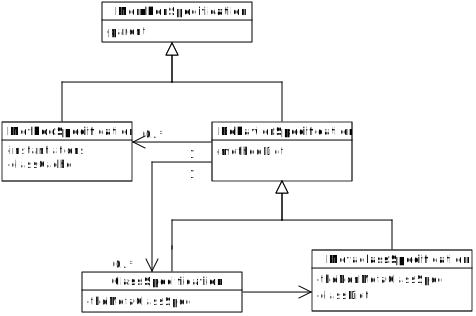
\includegraphics[scale=1]{metamodel.pdf}
	\caption{Meta Model for Nested Classes}
	\label{fig:impl_meta_model}
\end{figure}

\paragraph{Class Specifications}
A class specification describes classes. It has a collection of \texttt{MethodSpecification}s, representing instance methods of the class. Upon instantiation, all method specifications are instantiated within the target class. For every class specification, there is a corresponding method specification containing the source code of the class generator method in the parent's method dictionary. This method specification determines (when executed in the running system) to which class the methods will be added (\emph{target class}). Top-level classes are an exception: they are always a new subclass of the class \texttt{Module}.

\paragraph{Meta Class Specification}
A meta class specification describes meta classes. It has a collection of \texttt{MethodSpecification}s, representing class methods of the class (i.e., instance methods of the meta class). Upon instantiation, all method specifications are instantiated within the targer class' meta class. Consequently, meta classes do not method specifications associated with.

However, meta classes can have nested classes of their own. For every class defined in a meta class, there is a corresponding method specification present in the method dictionary (see previous paragraph).

\paragraph{Method Specification}
A method specification describes methods. It contains the source code of the method and stores information necessary for class caching and UI metadata. Whenever a method specification is instantiated, the method source code is compiled in the target class. 

Note, that different byte code must be generated for different target classes: for example, instance variable reads and write are compiled to parameterized\footnote{There are separate bytecodes for reading the first or second instance variable etc.} \texttt{pushRcvr:} and \texttt{popIntoRcvr:} bytecodes, where instance variables are referenced with their index\footnote{The first instance variable has index 0, second index variable has index 1, etc.}. In addition, the \texttt{outer} and the \texttt{enclosing} keyword must be bound to different method literals, depending on the lexical scope of the class.

\paragraph{Class Initialization}

accessor methods and generator methods, lazy initialization

\section{Anonymous Classes and Subclass Generation}

\section{\texttt{thisOuter} and \texttt{thisScope}}

\section{Class Updates}
using instances weak array on specification

\section{Integration in Squeak}

\subsection{Module Repository}
replacement for Smalltalk dict

\subsection{IDE Support}
works in workspace, test runner. How to write tests? New system browser

\subsection{Debugger}
shows slightly different code (thisContext automatically inserted, generator methods)
\chapter{Use Cases}

\section{Avoiding Clasds Name Clashes}
example: multiple games, all providing game class

\section{Module Versioning}
example: multiple versions of the same module in the same image

\section{Dependency Management}
example: app that requires a specific version (defining local alias), then all access goes through that method. example: external configuration of modules with parameterized classes (alternative to dependency injection)

\section{Readability and Understandability}
example: large project, where parts of the code can now be understood, given that we have hierarchical nesting. could be an example where grouping according to multiple criteria is needed (would result in n x m packages)

\section{Mixin Modularity with Parameterized Classes}

\section{Class Generator Pattern}
\label{sec:usecase_classgen}
better syntax for class generators

\section{Extension Methods}
better way is needed (e.g., class boxes, refinements, COP). return already existing class in generator method

\chapter{Future Work}
\label{sec:future}
In this section, we give an overview of possible areas of future work. We also point of deficiencies of \msname that we want to address in future versions.

\section{Classes as Instance-side Members}
\label{sec:future_inst_side}
Java and Newspeak support nested classes as instance-side members (non-static member classes). Earlier versions \msname included support for instance-side nested classes, but this caused difficulties in the implementation. 

\begin{itemize}
	\item \emph{Method lookup:} Classes can now be enclosed in instances instead of classes. We are not sure whether a message send to \texttt{enclosing}, \texttt{outer}, or \texttt{scope} should also lookup methods on the class side whenever a message was not understood on the instance side. It would certainly be good style to nest classes that do not need access to instance-specific state as class class-side members. These classes should then be accessible within an instance using an implicit receiver send or the \texttt{scope} keyword.
	\item \emph{\texttt{outer}/\texttt{enclosing} cannot be early bound:} These keyword might have to start their lookup in an instance. Therefore, these keywords cannot be bound as literals, which are stored in methods and, therefore, shared among all instances.
	\item \emph{Possible memory issues:} In contrast to Java, \msname would generate a new class every time an instance-side member class is accessed. This could lead to memory and performance issues.
\end{itemize}

In addition to these difficulties, we are currently unclear about what the exact benefits of instance-side nested classes are. They can be used to build mixins, but the we achieve the same functionality with parameterized classes (see Section~\ref{sec:rel_mixins1}). In Java, non-static member classes are used to implement interface adapters that need access to the enclosing instance~\cite{Bloch:2008:EJ:1377533} (see Section~\ref{sec:rel_ns_pkg_cls_nesting}). This is, however, the only pattern for non-static member classes we could find in literature, and the same functionality can be achieved by implementing the adapter as a class-side nested class with an instance variable holding a reference to the adaptee.

As a consequence, we removed support for instance-side nested classes, but we might add it again at a later point of time, if it needed.

\section{Bytecode Transformation}
Whenever a nested class specification is instantiated in \msname, all methods in the specification are complied in the target class. When using parameterized classes, this process happens multiple times, once for every target class. However, the bytecode is almost the same for every target class and differs only for reads/writes to instance variables (see Section~\ref{sec:impl_ch_inst_cl_vars}). In addition, \texttt{enclosing} and \texttt{outer} must be bound to different literals.

This process could be optimized by caching compiled methods and replacing affected bytecodes and literals during instantiation. For example, instead of recompiling the entire method, all references to instance variables could be replaced with bytecodes with the correct indices in a linear pass through the compiled method.

In Newspeak, slots (instance variables) cannot be accessed directly. They are always accessed through automatically-generated accessor methods. Therefore, all references to slots are message sends. Consequently, the bytecode of a method for two different instantiations is always the same.

\section{Squeak Integration}
As of now, the integration of \msname in Squeak is still limited. For example, the new class browser does not have any refactoring tools yet. Furthermore, all Squeak classes should be migrated to classes in \msname, eventually, making \texttt{Repository} (a separate \texttt{globals} dictionary for \msname) obsolete.

\section{Extension Methods}
\label{sec:future_ext_meth}
In Smalltalk, an extension method is a method that extends an already existing class in another package. Additional methods can be defined on the instance side and and on the class side. Adding new instance/class variables or removing methods is not supported. In \msname, extension methods can be written by defining a class extension: a nested class with a class generator method that returns an already existing class.

Extension methods in Smalltalk and in \msname are controversial because they do not have proper conflict handling. If an extension method is defined and the target class has already a method with the same name, the original method is replaced, possibly breaking other code. Extension methods can be used to add new functionality to existing classes required by libraries (e.g., methods for the visitor design pattern). If two libraries add extension methods with the same name, the second extension always wins. In addition, removing an extension method does not restore the previous state: the original method has to be restored manually by the programmer.

Smalltalk extension methods break modularity. It is not possible to compose two modules providing colliding extension methods, because there is currently no way to resolve method conflicts without changing the source code of at least one of the modules. Furthermore, modules providing extension methods are not easily replacable, because the original state is not restored once a module is removed from the system.

Other programming languages (e.g., Ruby) have a concept similar to extension methods in Smalltalk. A variety of alternatives to extension methods have been proposed. In the rest of this chapter, we give a brief overview of some of them. Future versions of \msname might incorporate one of these alternatives.

\paragraph{Classboxes}
A classbox is a container of classes and methods. Classes can either be defined or imported into a classbox (from another classbox). Within a classbox, additional methods can be added or replaced on imported classes (\emph{local rebinding}). Code executed in the context of certain classbox has a modified method lookup: the system tries to lookup methods defined in the classbox first, and then proceeds with the ordinary method lookup (receiver class and superclass hierarchy)~\cite{bergel:inria-00533446}.

A classbox effectively acts as a sort of sandbox. Every classbox can define its own extensions methods for imported classes. Duplicate extension methods are not a problem as long as they are defined in different classboxes. 

Implementations of classboxes exist for Squeak~\cite{bergel:inria-00533446} and Java. Classbox/J is a Java implementation which does not only allow redefining fields and methods but also member classes (nested/inner classes)~\cite{Bergel:2005:CCS:1094811.1094826}.

\paragraph{Ruby Refinements}
In Ruby, all classes and modules are open for extensions. At any position in the program, existing classes can be modified, possibly breaking other code. Refinements are a way to confine class/module extensions to certain classes. A refinement can be defined as part of a module. Whenever the module is included, the refinement is active for code written in the including class~\cite{Carlson:2015:RC:1212915}. Other code is not affected.

\paragraph{Context-oriented Programming}
Context-oriented programming (COP) is a mechanism to modularize heterogeneous crosscutting concerns~\cite{Hirschfeld08context-orientedprogramming}. In layer-based context oriented programming, crosscutting concerns are grouped in layers. A layer is a set of partial method definitions (possibly from different classes). Every partial method definition belongs to exactly one base method. Whenever a layer is active, the system executes the partial methods defined in the layer instead of the corresponding base methods. Multiple layers can be active at the same time, effectively building a layer composition stack. A partial method can contain a \texttt{proceed} statement, which will call the next partial method, i.e., the partial method defined in the next layer on the layer composition stack. If there is no next layer defining a partial method for the corresponding base method, the system will call the base method.

Every module could group its extension methods in a separate layer, activate that layer whenever code from the module is run, and deactivate the layer afterwards. Most COP implementations support scoped layer activation~\cite{Appeltauer:2009:CCP:1562112.1562118}, which essentially activates a layer, then runs a method or function/block closure, and then deactivates the layer again.

With context-oriented programming, duplicate extension methods are no longer a problem, as long as they are contained in different layers as partial method definitions.

%\paragraph{Worlds}
%better way is needed (e.g., class boxes, refinements, COP, world (paper viewpoints), monkey patching). return already existing class in generator method

\section{Extending Inherited Nested Classes without Subclassing}
The way inherited nested classes can be extended without subclassing has two deficiencies. Firstly, there is currently no notation to add new instance variables to the extended class, because the subclass statement is part of the corresponding method in the superclass. Secondly, nested classes of already extended classes cannot be further extended, because a \texttt{super} call would not call the original class accessor method. Instead, the method lookup would start in the superclass of extended class (which is the same class as the not yet extended class).

It is still unclear, if extending inherited nested classes without subclassing should be forbidden in favor of the variant \emph{with subclassing}. Other programming languages like Jx do this by default~\cite{Nystrom:2004:SEV:1028976.1028986}. Extending inherited nested classes with subclassing would solve the problems described above and is already possible. However, forbidding \emph{extending without subclassing} is difficult without restricting the ability to write extension methods, which is technically a very similar concept.

\section{Dependency Management}
Nested classes in \msname can be used to store modules in different versions. There is at the moment no convenient way to share modules with other developers, except for exporting the module and importing it again. Future versions of \msname might have a central remote repository from which modules are automatically downloaded (similar to a Maven repository) if a module is referenced that is available in the image. The corresponding functionality could be part of a \texttt{doesNotUnderstand:} handler in \texttt{Repository}, which is the data structure holding references to all modules installed in the image.

There are also ideas for a better integration of the underlying source code management system (e.g., git) in \msname. If \msname is aware of commits, it can not only be used to run applications in certain versions, but also to run applications at a certain commit. Whether the source code management system should be completely reimplemented in \msname or be external and under control of \msname is still open to discussion.

% automatically download dependencies
% generate list of all dependencies

%\blinddocument

\printbibliography
\clearpage
\appendix
%% ggf:
% \part{Appendix}
% \label{part:appendix}

\chapter{Implementation Details}

\section{Determining the Lexical Scope}
\label{sec:app_lexical_scope}

\section{Traits}
\label{sec:app_traits}

%%% Local Variables: 
%%% mode: latex
%%% End: 

\backmatter
\markboth{}\relax

% BAMA-O (2009) §24.8
%  Am Schluss der Arbeit hat die/der Kandidat/in  zu versichern, dass 
%  sie/er sie selbstständig verfasst sowie keine anderen Quellen und 
%  Hilfsmittel als die angegebenen benutzt hat.
% BAMA-O (2013) §30.6
%  Am Schluss der Arbeit hat die Kandidatin bzw. der Kandidat zu versichern,
%  dass sie bzw. er die Arbeit selbstständig verfasst und keine anderen
%  Quellen und Hilfsmittel als die angegebenen benutzt hat.
\defaultstatement
\end{document}
%%% Local Variables:
%%% mode: latex
%%% TeX-master: t
%%% End:
